% Appendix of the LoCoBench dataset paper.

%% ============================================================================
\section{The Pipeline's Prompts, Verbatim}
\label{app:prompts}
%% ============================================================================

Every prompt below is exported from the pipeline's code by
\texttt{scripts/locobench\_export\_prompts.py}, so it is the text that was sent.
\texttt{[\ldots\_PLACEHOLDER]} marks where the pipeline substitutes a value. Prompts in the
function-call idiom (V3, V4, SV1, SV5) follow the committee format of LoReFact \citep{lorefact}:
the model is asked to evaluate a Python call and return JSON.

\subsection{Generation}

\paragraph{P1: topic to question.}
\promptfile{prompts/PROMPT_P1.txt}

\paragraph{P2: question to tagged claim pool.}
\promptfile{prompts/PROMPT_P2.txt}

\paragraph{S3: claims to slot plan.} \texttt{[SENSES\_PLACEHOLDER]} receives the family's one or
two rare senses; \texttt{[SLOTS\_PLACEHOLDER]} receives the slot requirement of its primary ladder
type, given after the prompt.
\promptfile{prompts/PROMPT_S3.txt}

\noindent Slot requirement, \cp{conflict}:
\promptfile{prompts/INSERT_S3_SLOTS_CONFLICT.txt}
\noindent Slot requirement, \cp{chain}:
\promptfile{prompts/INSERT_S3_SLOTS_CHAIN.txt}
\noindent Slot requirement, \cp{sign}:
\promptfile{prompts/INSERT_S3_SLOTS_SIGN.txt}
\noindent Slot requirement, \cp{order}:
\promptfile{prompts/INSERT_S3_SLOTS_ORDER.txt}

\paragraph{S4: plan to template and fillers.} \texttt{[LAYOUT\_PLACEHOLDER]} receives
``Organize the answer into 3-5 paragraphs.'' for \cp{conflict}, \cp{chain} and \cp{sign}, and for
\cp{order}:
\promptfile{prompts/INSERT_S4_LAYOUT_ORDER.txt}
\promptfile{prompts/PROMPT_S4.txt}

\paragraph{SF: regenerating one filler.}
\promptfile{prompts/PROMPT_SF.txt}

\paragraph{Retry notes.} Appended to a prompt whose output failed to parse, or failed a
deterministic check, together with the reason:
\promptfile{prompts/RETRY_PARSE.txt}
\promptfile{prompts/RETRY_SEMANTIC.txt}

\subsection{Committee}

\paragraph{V3: fluency, leakage, hedging, artifacts.}
\promptfile{prompts/PROMPT_V3.txt}

\paragraph{V4: claim coverage.}
\promptfile{prompts/PROMPT_V4.txt}

\paragraph{SV1: blind pair-by-pair relation reading.}
\promptfile{prompts/PROMPT_SV1.txt}

\paragraph{SV5: blind filler reading.}
\promptfile{prompts/PROMPT_SV5.txt}

\subsection{Reference Evaluation}

The prompts of the companion paper's relation miners and LLM judges (\S\ref{sec:reference}).

\paragraph{Graph-level miner.}
\promptfile{prompts/EVAL_GRAPH_MINER.txt}

\paragraph{Pairwise miner, Prompt A (sense and coupling).}
\promptfile{prompts/EVAL_PAIR_A.txt}

\paragraph{Pairwise miner, Prompt B (strength).}
\promptfile{prompts/EVAL_PAIR_B.txt}

\paragraph{G-Eval coherence judge.}
\promptfile{prompts/EVAL_JUDGE_GEVAL.txt}

\paragraph{Direct 1--5 coherence rating.}
\promptfile{prompts/EVAL_JUDGE_DIRECT.txt}

%% ============================================================================
\section{Worked Families}
\label{app:families}
%% ============================================================================

One family of each primary ladder type, extracted from the release by
\texttt{scripts/locobench\_paper\_examples.py}. Each lists the question, the plan's claims with
their labels, the template with its slot markers, every slot's fillers, the five responses with
the filler each carries in the edited slots and its gold $\LCS$ at both worlds, one response in
full with its slot sentences highlighted, and that response's gold relations. The other responses
are the template with the listed fillers spliced in.

\subsection{A \cp{conflict} family (f009)}
% Generated by scripts/locobench_paper_examples.py from f009.
\paragraph{Question.} How do engineers establish whether an intermittent failure in a large distributed system originates in application logic or in the underlying hardware, when the postmortem evidence initially supports two competing accounts? (Computer Science, Engineering \& Technology.)

\paragraph{Claims.} The plan's claims in assertion order, with their factuality labels; claims joined by a ladder's slots are boxed.

\begin{center}\scriptsize
\setlength{\tabcolsep}{2.5pt}
\begin{tabular}{@{}rp{0.76\linewidth}l@{}}
\toprule
& Claim & Label \\
\midrule
\slotclaim{$a_{1}$} & Platform telemetry recorded machine check exceptions on several hosts in the cluster. & true \\
\slotclaim{$a_{2}$} & The failures persisted on hosts whose memory modules had been freshly replaced. & true \\
\slotclaim{$a_{3}$} & The ECC subsystem logged correctable single-bit errors on two hosts during the incident window. & true \\
\slotclaim{$a_{4}$} & Hardware faults typically cluster on individual machines rather than following a single code path. & true \\
$a_{5}$ & ECC memory silently corrects double-bit errors without recording any event. & \textbf{false} \\
$a_{6}$ & A subset of the cluster's memory modules produced uncorrectable errors. & true \\
$a_{7}$ & The application accessed shared state without synchronization. & true \\
$a_{8}$ & The corrupted responses carried checksums that did not match their payloads. & true \\
$a_{9}$ & The suspect code path used a lock-free ring buffer shared between worker threads. & true \\
\slotclaim{$a_{10}$} & A thread-sanitizer build reported a data race on the ring buffer's write index. & true \\
\slotclaim{$a_{11}$} & The remediation added a memory barrier around updates to the shared write index. & true \\
$a_{12}$ & Hardware-induced faults reproduce deterministically on every execution of the same code path. & \textbf{false} \\
$a_{13}$ & Corrupted responses appeared only on hosts running the new application release. & true \\
$a_{14}$ & No host running the previous application release produced a corrupted response. & true \\
\bottomrule
\end{tabular}
\end{center}

\paragraph{Template.} The answer as written once, with its slot markers.

\begin{quote}\small
Resolving a dispute of this kind depends less on gathering more evidence than on locating the single observation that only one of the two accounts can accommodate. The standard first move is therefore to audit the platform layer, because a hardware story and a software story predict different distributions of symptoms across machines, releases and code paths. \slotmarker{S1}

\slotmarker{S2} Although correctable errors were logged during that window, ECC memory silently corrects double-bit errors without recording any event, so a sparse log is not by itself a clean bill of health. The machine check exceptions captured across the cluster nevertheless show that a subset of the cluster's memory modules produced uncorrectable errors; the continued failure of hosts whose memory had just been swapped out, by contrast, tells against reading the incident as a pure component defect. At that stage at least one of two conditions had to obtain, and perhaps both held together: uncorrectable errors in the cluster's memory, or an application that accessed shared state without synchronization.

The next step is to interrogate the corrupted output itself and the code that produced it. \slotmarker{S3} It was the unsynchronized sharing of that ring buffer across workers that produced the race condition instrumentation went on to detect. \slotmarker{S4} That sanitizer result confirms the second of the two candidate conditions, namely that the application was reaching shared state without the synchronization its correctness required.

The decisive discrimination comes from the pattern of occurrence rather than from any single log entry. Hardware-induced faults reproduce deterministically on every execution of the same code path; the corrupted responses, by contrast, appeared only on hosts running the new application release. That is, no host running the previous application release produced a corrupted response. The method, in summary, is to treat each account as a prediction about where symptoms should and should not appear, to find the boundary at which one prediction fails, and then to replace inference from telemetry with direct instrumentation of the suspect path.
\end{quote}

\paragraph{Fillers.} Each slot's fillers, as admitted by the committee.

\begin{center}\scriptsize
\setlength{\tabcolsep}{2.5pt}
\begin{tabular}{@{}lp{0.80\linewidth}@{}}
\toprule
Filler & Text \\
\midrule
\multicolumn{2}{@{}l}{\slotmarker{S1} conflict slot, $a_{1}$--$a_{2}$} \\
\quad conflict & Platform telemetry recorded machine check exceptions on several hosts in the cluster, a record that cannot be squared with the persistence of the failures on hosts whose memory modules had been freshly replaced. \\
\quad no link & Platform telemetry recorded machine check exceptions on several hosts in the cluster. The failures persisted on hosts whose memory modules had been freshly replaced. \\
\addlinespace
\multicolumn{2}{@{}l}{\slotmarker{S2} conflict slot, $a_{3}$--$a_{4}$} \\
\quad conflict & The ECC subsystem logged correctable single-bit errors on two hosts during the incident window, a signature that cannot be squared with the fact that hardware faults typically cluster on individual machines rather than following a single code path. \\
\quad no link & The ECC subsystem logged correctable single-bit errors on two hosts during the incident window. As a general matter, hardware faults typically cluster on individual machines rather than following a single code path. \\
\addlinespace
\multicolumn{2}{@{}l}{\slotmarker{S3} conflict (spare) slot, $a_{8}$--$a_{9}$} \\
\quad conflict & The corrupted responses carried checksums that did not match their payloads, which rules out the possibility that the suspect code path used a lock-free ring buffer shared between worker threads, as it did. \\
\quad no link & The corrupted responses carried checksums that did not match their payloads. The suspect code path used a lock-free ring buffer shared between worker threads. \\
\addlinespace
\multicolumn{2}{@{}l}{\slotmarker{S4} control slot, $a_{10}$--$a_{11}$} \\
\quad wording 1 & A thread-sanitizer build reported a data race on the ring buffer's write index, and that report led directly to a remediation that added a memory barrier around updates to the shared write index. \\
\quad wording 2 & Because a thread-sanitizer build reported a data race on the ring buffer's write index, the remediation added a memory barrier around updates to the shared write index. \\
\quad wording 3 & The remediation added a memory barrier around updates to the shared write index, a change brought about by a thread-sanitizer build's report of a data race on the ring buffer's write index. \\
\bottomrule
\end{tabular}
\end{center}

\paragraph{Rungs.} The five responses of the family, which filler each carries in the edited slots, and gold $\LCS$ at the verdict and the asserted world.

\begin{center}\scriptsize
\setlength{\tabcolsep}{2.5pt}
\begin{tabular}{@{}l>{\raggedright\arraybackslash}p{0.27\linewidth}>{\raggedright\arraybackslash}p{0.30\linewidth}cc@{}}
\toprule
& Ladder, rung & Fillers & \multicolumn{2}{c}{$\LCS$ at world} \\
& & & verdict & asserted \\
\midrule
t0 & conflict $\rho_0$ & S1: conflict, S2: conflict & 0.151 & 0.151 \\
t1 & conflict $\rho_1$, control $\rho_0$ & S1: conflict, S2: no link & 0.343 & 0.343 \\
t2 & conflict $\rho_2$ & S1: no link, S2: no link & 0.849 & 0.849 \\
t3 & control $\rho_1$ & S4: wording 2 & 0.343 & 0.343 \\
t4 & control $\rho_2$ & S4: wording 3 & 0.343 & 0.343 \\
\bottomrule
\end{tabular}
\end{center}

\paragraph{Response t1 in full} (conflict $\rho_1$; edited slots highlighted, 447 words).

\begin{quote}\small
Resolving a dispute of this kind depends less on gathering more evidence than on locating the single observation that only one of the two accounts can accommodate. The standard first move is therefore to audit the platform layer, because a hardware story and a software story predict different distributions of symptoms across machines, releases and code paths. \slotfill{S1}{Platform telemetry recorded machine check exceptions on several hosts in the cluster, a record that cannot be squared with the persistence of the failures on hosts whose memory modules had been freshly replaced.}

\slotfill{S2}{The ECC subsystem logged correctable single-bit errors on two hosts during the incident window. As a general matter, hardware faults typically cluster on individual machines rather than following a single code path.} Although correctable errors were logged during that window, ECC memory silently corrects double-bit errors without recording any event, so a sparse log is not by itself a clean bill of health. The machine check exceptions captured across the cluster nevertheless show that a subset of the cluster's memory modules produced uncorrectable errors; the continued failure of hosts whose memory had just been swapped out, by contrast, tells against reading the incident as a pure component defect. At that stage at least one of two conditions had to obtain, and perhaps both held together: uncorrectable errors in the cluster's memory, or an application that accessed shared state without synchronization.

The next step is to interrogate the corrupted output itself and the code that produced it. The corrupted responses carried checksums that did not match their payloads. The suspect code path used a lock-free ring buffer shared between worker threads. It was the unsynchronized sharing of that ring buffer across workers that produced the race condition instrumentation went on to detect. \slotfill{S4}{A thread-sanitizer build reported a data race on the ring buffer's write index, and that report led directly to a remediation that added a memory barrier around updates to the shared write index.} That sanitizer result confirms the second of the two candidate conditions, namely that the application was reaching shared state without the synchronization its correctness required.

The decisive discrimination comes from the pattern of occurrence rather than from any single log entry. Hardware-induced faults reproduce deterministically on every execution of the same code path; the corrupted responses, by contrast, appeared only on hosts running the new application release. That is, no host running the previous application release produced a corrupted response. The method, in summary, is to treat each account as a prediction about where symptoms should and should not appear, to find the boundary at which one prediction fails, and then to replace inference from telemetry with direct instrumentation of the suspect path.
\end{quote}

\paragraph{Gold relations of response t1.} Sense, compiled coupling, strength band, and the relation's sign at the verdict (v.) and asserted (a.) world ($+$ support, $-$ conflict, $\cdot$ no factor); a slot id marks a relation drawn by a filler.

\begin{center}\scriptsize
\setlength{\tabcolsep}{2.2pt}
\begin{tabular}{@{}lllllcc@{}}
\toprule
Pair & & Sense & Coupling & Band & v. & a. \\
\midrule
$a_{1}\to a_{2}$ & S1 & Refutation & contradiction & strong & $-$ & $-$ \\
$a_{1}\to a_{6}$ &  & Evidence & entailment & moderate & $+$ & $+$ \\
$a_{2}\to a_{6}$ &  & Contrast & none & moderate & $\cdot$ & $\cdot$ \\
$a_{3}\to a_{5}$ &  & Concession & none & moderate & $\cdot$ & $\cdot$ \\
$a_{6}\to a_{7}$ &  & Disjunction & co-necessity & strong & $+$ & $+$ \\
$a_{9}\to a_{10}$ &  & Cause-Effect & entailment & moderate & $+$ & $+$ \\
$a_{10}\to a_{7}$ &  & Evidence & entailment & strong & $+$ & $+$ \\
$a_{10}\to a_{11}$ & S4 & Cause-Effect & entailment & strong & $+$ & $+$ \\
$a_{12}\to a_{13}$ &  & Contrast & none & moderate & $\cdot$ & $\cdot$ \\
$a_{13}\to a_{14}$ &  & Restatement & equivalence & strong & $+$ & $+$ \\
\bottomrule
\end{tabular}
\end{center}


\subsection{A \cp{chain} family (f224)}
% Generated by scripts/locobench_paper_examples.py from f224.
\paragraph{Question.} How do economists adjudicate between the claim that the 1970s stagflation originated in oil supply shocks and the claim that it originated in monetary policy errors, and what evidence settled the dispute? (Economics, Social Sciences.)

\paragraph{Claims.} The plan's claims in assertion order, with their factuality labels; claims joined by a ladder's slots are boxed.

\begin{center}\scriptsize
\setlength{\tabcolsep}{2.5pt}
\begin{tabular}{@{}rp{0.76\linewidth}l@{}}
\toprule
& Claim & Label \\
\midrule
\slotclaim{$a_{1}$} & OPEC imposed an oil embargo on the United States in October 1973. & true \\
\slotclaim{$a_{2}$} & The price of crude oil roughly quadrupled between 1973 and early 1974. & true \\
\slotclaim{$a_{3}$} & Hamilton documented a statistical relationship between oil price increases and postwar US recessions. & true \\
$a_{4}$ & Oil supply shocks account for the entire rise in US inflation during the 1970s. & \textbf{false} \\
$a_{5}$ & US consumer price inflation exceeded 5 percent before the October 1973 oil embargo. & true \\
$a_{6}$ & US consumer price inflation remained below 5 percent until the October 1973 oil embargo. & true \\
$a_{7}$ & OPEC production cuts sharply raised the real price of crude oil in 1973 and 1974. & true \\
$a_{8}$ & US money growth accelerated in the years preceding 1973. & true \\
$a_{9}$ & Japan experienced lower consumer price inflation than the United States in 1974. & \textbf{false} \\
$a_{10}$ & The Federal Reserve's policy interest rate stood below the rate of inflation for much of the 1970s. & true \\
$a_{11}$ & Real policy interest rates in the United States were negative during much of the 1970s. & true \\
$a_{12}$ & Clarida, Gali and Gertler estimated that the pre-1979 Federal Reserve policy rule violated the Taylor principle. & true \\
\slotclaim{$a_{13}$} & Paul Volcker became chairman of the Federal Reserve in August 1979. & true \\
\slotclaim{$a_{14}$} & The Volcker tightening pushed the federal funds rate above 19 percent in 1981. & true \\
\bottomrule
\end{tabular}
\end{center}

\paragraph{Template.} The answer as written once, with its slot markers.

\begin{quote}\small
Adjudicating between the supply-shock and the monetary-policy accounts of the 1970s turns on timing, on cross-country comparison, and on the estimated behaviour of the central bank's reaction function. \slotmarker{S1} \slotmarker{S2} That recession regularity indicates that oil supply shocks account for the entire rise in US inflation during the 1970s.

The chronology, however, disciplines any such attribution. Only two descriptions of the pre-embargo record are available, and exactly one of them can be correct: either US consumer price inflation exceeded 5 percent before the October 1973 oil embargo, or it remained below 5 percent until that embargo. The published price indices place the decade in the first case, and inflation already above 5 percent in advance of the embargo cannot be squared with the view that oil supply shocks produced the whole of the decade's inflation. What can be affirmed is that at least one of two impulses was in operation, and perhaps both were: OPEC production cuts sharply raised the real price of crude oil in 1973 and 1974, and US money growth accelerated in the years preceding 1973.

The monetary side of the ledger rests on further evidence. Japan experienced lower consumer price inflation than the United States in 1974. The Federal Reserve's policy interest rate stood below the rate of inflation for much of the 1970s; in other words, real policy interest rates in the United States were negative during much of the decade, and the Japanese comparison for 1974 is precisely the sort of international evidence that shows those American real rates to have been negative. That sustained shortfall of real rates below zero is in turn evidence for the estimate of Clarida, Gali and Gertler that the pre-1979 Federal Reserve policy rule violated the Taylor principle: a central bank that raises its nominal rate by less than one-for-one with inflation will let real rates fall as prices accelerate.

The dispute was settled less by any single regression than by an institutional experiment at the close of the decade. \slotmarker{S3} The lesson drawn from that episode is that a determined central bank can end an inflation whose proximate trigger lay in commodity markets, and the weight of professional judgment shifted accordingly toward the monetary account.
\end{quote}

\paragraph{Fillers.} Each slot's fillers, as admitted by the committee.

\begin{center}\scriptsize
\setlength{\tabcolsep}{2.5pt}
\begin{tabular}{@{}lp{0.80\linewidth}@{}}
\toprule
Filler & Text \\
\midrule
\multicolumn{2}{@{}l}{\slotmarker{S1} chain link slot, $a_{1}$--$a_{2}$} \\
\quad support & OPEC imposed an oil embargo on the United States in October 1973, and that embargo caused the price of crude oil to roughly quadruple between 1973 and early 1974. \\
\quad no link & OPEC imposed an oil embargo on the United States in October 1973. The price of crude oil, which can be traced through posted contract terms, roughly quadrupled between 1973 and early 1974. \\
\addlinespace
\multicolumn{2}{@{}l}{\slotmarker{S2} chain link slot, $a_{2}$--$a_{3}$} \\
\quad support & A quadrupling of that magnitude confirms the statistical relationship Hamilton documented between oil price increases and postwar US recessions. \\
\quad no link & Hamilton, working through the postwar US record, documented a statistical relationship between oil price increases and recessions. \\
\addlinespace
\multicolumn{2}{@{}l}{\slotmarker{S3} control slot, $a_{13}$--$a_{14}$} \\
\quad wording 1 & Paul Volcker became chairman of the Federal Reserve in August 1979, and his arrival led to a tightening that pushed the federal funds rate above 19 percent in 1981. \\
\quad wording 2 & The federal funds rate was driven above 19 percent in 1981 by the tightening that resulted from Paul Volcker's accession to the chairmanship of the Federal Reserve in August 1979. \\
\quad wording 3 & Because Paul Volcker took charge of the Federal Reserve as chairman in August 1979, a tightening followed that carried the federal funds rate past 19 percent in 1981. \\
\bottomrule
\end{tabular}
\end{center}

\paragraph{Rungs.} The five responses of the family, which filler each carries in the edited slots, and gold $\LCS$ at the verdict and the asserted world.

\begin{center}\scriptsize
\setlength{\tabcolsep}{2.5pt}
\begin{tabular}{@{}l>{\raggedright\arraybackslash}p{0.27\linewidth}>{\raggedright\arraybackslash}p{0.30\linewidth}cc@{}}
\toprule
& Ladder, rung & Fillers & \multicolumn{2}{c}{$\LCS$ at world} \\
& & & verdict & asserted \\
\midrule
t0 & chain $\rho_0$ & S1: no link, S2: no link & 0.337 & 0.067 \\
t1 & chain $\rho_1$, control $\rho_0$ & S1: support, S2: no link & 0.398 & 0.086 \\
t2 & chain $\rho_2$ & S1: support, S2: support & 0.478 & 0.115 \\
t3 & control $\rho_1$ & S3: wording 2 & 0.398 & 0.086 \\
t4 & control $\rho_2$ & S3: wording 3 & 0.398 & 0.086 \\
\bottomrule
\end{tabular}
\end{center}

\paragraph{Response t1 in full} (chain $\rho_1$; edited slots highlighted, 440 words).

\begin{quote}\small
Adjudicating between the supply-shock and the monetary-policy accounts of the 1970s turns on timing, on cross-country comparison, and on the estimated behaviour of the central bank's reaction function. \slotfill{S1}{OPEC imposed an oil embargo on the United States in October 1973, and that embargo caused the price of crude oil to roughly quadruple between 1973 and early 1974.} \slotfill{S2}{Hamilton, working through the postwar US record, documented a statistical relationship between oil price increases and recessions.} That recession regularity indicates that oil supply shocks account for the entire rise in US inflation during the 1970s.

The chronology, however, disciplines any such attribution. Only two descriptions of the pre-embargo record are available, and exactly one of them can be correct: either US consumer price inflation exceeded 5 percent before the October 1973 oil embargo, or it remained below 5 percent until that embargo. The published price indices place the decade in the first case, and inflation already above 5 percent in advance of the embargo cannot be squared with the view that oil supply shocks produced the whole of the decade's inflation. What can be affirmed is that at least one of two impulses was in operation, and perhaps both were: OPEC production cuts sharply raised the real price of crude oil in 1973 and 1974, and US money growth accelerated in the years preceding 1973.

The monetary side of the ledger rests on further evidence. Japan experienced lower consumer price inflation than the United States in 1974. The Federal Reserve's policy interest rate stood below the rate of inflation for much of the 1970s; in other words, real policy interest rates in the United States were negative during much of the decade, and the Japanese comparison for 1974 is precisely the sort of international evidence that shows those American real rates to have been negative. That sustained shortfall of real rates below zero is in turn evidence for the estimate of Clarida, Gali and Gertler that the pre-1979 Federal Reserve policy rule violated the Taylor principle: a central bank that raises its nominal rate by less than one-for-one with inflation will let real rates fall as prices accelerate.

The dispute was settled less by any single regression than by an institutional experiment at the close of the decade. \slotfill{S3}{Paul Volcker became chairman of the Federal Reserve in August 1979, and his arrival led to a tightening that pushed the federal funds rate above 19 percent in 1981.} The lesson drawn from that episode is that a determined central bank can end an inflation whose proximate trigger lay in commodity markets, and the weight of professional judgment shifted accordingly toward the monetary account.
\end{quote}

\paragraph{Gold relations of response t1.} Sense, compiled coupling, strength band, and the relation's sign at the verdict (v.) and asserted (a.) world ($+$ support, $-$ conflict, $\cdot$ no factor); a slot id marks a relation drawn by a filler.

\begin{center}\scriptsize
\setlength{\tabcolsep}{2.2pt}
\begin{tabular}{@{}lllllcc@{}}
\toprule
Pair & & Sense & Coupling & Band & v. & a. \\
\midrule
$a_{1}\to a_{2}$ & S1 & Cause-Effect & entailment & strong & $+$ & $+$ \\
$a_{3}\to a_{4}$ &  & Evidence & entailment & weak & $-$ & $+$ \\
$a_{5}\to a_{4}$ &  & Refutation & contradiction & strong & $+$ & $-$ \\
$a_{5}\to a_{6}$ &  & Alternative & exclusive & strong & $-$ & $-$ \\
$a_{7}\to a_{8}$ &  & Disjunction & co-necessity & strong & $+$ & $+$ \\
$a_{9}\to a_{11}$ &  & Evidence & entailment & weak & $+$ & $+$ \\
$a_{10}\to a_{11}$ &  & Restatement & equivalence & strong & $+$ & $+$ \\
$a_{11}\to a_{12}$ &  & Evidence & entailment & moderate & $+$ & $+$ \\
$a_{13}\to a_{14}$ & S3 & Cause-Effect & entailment & strong & $+$ & $+$ \\
\bottomrule
\end{tabular}
\end{center}


\subsection{A \cp{sign} family (f003)}
% Generated by scripts/locobench_paper_examples.py from f003.
\paragraph{Question.} How did astronomers establish whether the ``Great Debate'' nebulae lay within the Milky Way or formed separate galaxies, and what evidence ultimately settled the dispute? (Astronomy, Natural Sciences.)

\paragraph{Claims.} The plan's claims in assertion order, with their factuality labels; claims joined by a ladder's slots are boxed.

\begin{center}\scriptsize
\setlength{\tabcolsep}{2.5pt}
\begin{tabular}{@{}rp{0.76\linewidth}l@{}}
\toprule
& Claim & Label \\
\midrule
$a_{1}$ & The Great Debate was held on 26 April 1920 at the Smithsonian Museum of Natural History in Washington, D.C. & true \\
$a_{2}$ & Harlow Shapley argued that the spiral nebulae were gaseous clouds lying inside a single large Milky Way system. & true \\
$a_{3}$ & Heber Curtis argued that the spiral nebulae were distant stellar systems comparable in size to the Milky Way. & true \\
\slotclaim{$a_{4}$} & Curtis cited novae observed in spiral nebulae as evidence that those nebulae lay at great distances. & true \\
\slotclaim{$a_{5}$} & Curtis's analysis of novae in spiral nebulae placed M31 about 10,000 light years from the Sun. & \textbf{false} \\
$a_{6}$ & S Andromedae, which appeared in 1885, was a supernova far more luminous than an ordinary nova. & true \\
$a_{7}$ & Shapley relied on Adriaan van Maanen's reported measurements of internal rotation in spiral nebulae. & true \\
$a_{8}$ & Van Maanen's measurements of rotation in spiral nebulae were confirmed by later photographic plate comparisons. & \textbf{false} \\
$a_{9}$ & A later reexamination of van Maanen's plates concluded that the reported rotations of spiral nebulae were measurement artifacts. & true \\
$a_{10}$ & Henrietta Leavitt established the period-luminosity relation from Cepheid variables in the Magellanic Clouds. & true \\
\slotclaim{$a_{11}$} & Edwin Hubble identified Cepheid variable stars in M31 using the 100-inch Hooker telescope at Mount Wilson. & true \\
\slotclaim{$a_{12}$} & Hubble derived a distance to M31 of roughly 900,000 light years. & true \\
$a_{13}$ & M31 lies outside the boundaries of the Milky Way system. & true \\
$a_{14}$ & M31 lies within the boundaries of the Milky Way system. & true \\
\bottomrule
\end{tabular}
\end{center}

\paragraph{Template.} The answer as written once, with its slot markers.

\begin{quote}\small
The status of the spiral nebulae was first contested in open argument and only afterwards resolved by measurement. The Great Debate was held on 26 April 1920 at the Smithsonian Museum of Natural History in Washington, D.C. Harlow Shapley argued that the spiral nebulae were gaseous clouds lying inside a single large Milky Way system, whereas Heber Curtis argued that the spiral nebulae were distant stellar systems comparable in size to the Milky Way. The issue therefore turned on distance, and distance could be extracted only from objects of known intrinsic brightness.

\slotmarker{S1} By contrast, S Andromedae, which appeared in 1885, was a supernova far more luminous than an ordinary nova. The two classes of outburst were not yet separated in the photometry then available, so the eruptions recorded in the spirals could not yet be made to yield a secure scale.

Shapley's case for a single, all-encompassing system rested on evidence of a quite different kind, namely apparent motion within the spirals themselves, since a nebula visibly turning on a human timescale would have to be small and close at hand. \slotmarker{S2} A later reexamination of van Maanen's plates concluded that the reported rotations of spiral nebulae were measurement artifacts, and that verdict cannot be squared with any claim that subsequent comparisons of photographic plates had confirmed those rotations.

Resolution came from a calibrated distance indicator rather than from debate. Earlier, Henrietta Leavitt established the period-luminosity relation from Cepheid variables in the Magellanic Clouds; the search for such stars in the spirals came only afterwards. \slotmarker{S3} A figure of that magnitude demonstrates that M31 lies outside the boundaries of the Milky Way system. The two placements exclude one another: either M31 lies beyond the Galaxy's confines, or M31 lies within the boundaries of the Milky Way system, and exactly one of these must hold. On the Cepheid evidence, the spirals are stellar systems in their own right.
\end{quote}

\paragraph{Fillers.} Each slot's fillers, as admitted by the committee.

\begin{center}\scriptsize
\setlength{\tabcolsep}{2.5pt}
\begin{tabular}{@{}lp{0.80\linewidth}@{}}
\toprule
Filler & Text \\
\midrule
\multicolumn{2}{@{}l}{\slotmarker{S1} sign slot, $a_{4}$--$a_{5}$} \\
\quad conflict & Curtis cited novae observed in spiral nebulae as evidence that those nebulae lay at great distances; that evidence indicates a remove for M31 of about 10,000 light years from the Sun, the figure his analysis of those novae yielded. \\
\quad no link & Curtis cited novae observed in spiral nebulae as evidence that those nebulae lay at great distances. His analysis of novae in spiral nebulae placed M31 about 10,000 light years from the Sun. \\
\quad support & Curtis cited novae observed in spiral nebulae as evidence that those nebulae lay at great distances, and that evidence rules out the claim, sometimes attached to his analysis of novae in spiral nebulae, that it placed M31 about 10,000 light years from the Sun. \\
\addlinespace
\multicolumn{2}{@{}l}{\slotmarker{S2} sign (spare) slot, $a_{7}$--$a_{8}$} \\
\quad conflict & Shapley relied on Adriaan van Maanen's reported measurements of internal rotation in spiral nebulae, and that reliance shows that the rotations van Maanen reported were confirmed by later comparisons of photographic plates. \\
\quad no link & Shapley relied on Adriaan van Maanen's reported measurements of internal rotation in spiral nebulae. The rotations van Maanen reported were confirmed by later comparisons of photographic plates. \\
\quad support & Shapley relied on Adriaan van Maanen's reported measurements of internal rotation in spiral nebulae, and because nothing beyond those original reports of rotation stood behind the figures, the rotations cannot have been confirmed by later comparisons of photographic plates. \\
\addlinespace
\multicolumn{2}{@{}l}{\slotmarker{S3} control slot, $a_{11}$--$a_{12}$} \\
\quad wording 1 & Edwin Hubble identified Cepheid variable stars in M31 using the 100-inch Hooker telescope at Mount Wilson, and that identification led him to a distance for the nebula of roughly 900,000 light years. \\
\quad wording 2 & Because Edwin Hubble was able to pick out Cepheid variable stars in M31 with the 100-inch Hooker telescope at Mount Wilson, a distance of roughly 900,000 light years followed for that nebula. \\
\quad wording 3 & A distance to M31 of roughly 900,000 light years was the direct result of Edwin Hubble's detection of Cepheid variable stars in that nebula with the 100-inch Hooker telescope at Mount Wilson. \\
\bottomrule
\end{tabular}
\end{center}

\paragraph{Rungs.} The five responses of the family, which filler each carries in the edited slots, and gold $\LCS$ at the verdict and the asserted world.

\begin{center}\scriptsize
\setlength{\tabcolsep}{2.5pt}
\begin{tabular}{@{}l>{\raggedright\arraybackslash}p{0.27\linewidth}>{\raggedright\arraybackslash}p{0.30\linewidth}cc@{}}
\toprule
& Ladder, rung & Fillers & \multicolumn{2}{c}{$\LCS$ at world} \\
& & & verdict & asserted \\
\midrule
t0 & sign $\rho_0$ & S1: conflict & 0.123 & 0.036 \\
t1 & sign $\rho_1$, control $\rho_0$ & S1: no link & 0.292 & 0.030 \\
t2 & sign $\rho_2$ & S1: support & 0.334 & 0.036 \\
t3 & control $\rho_1$ & S3: wording 2 & 0.292 & 0.030 \\
t4 & control $\rho_2$ & S3: wording 3 & 0.292 & 0.030 \\
\bottomrule
\end{tabular}
\end{center}

\paragraph{Response t1 in full} (sign $\rho_1$; edited slots highlighted, 406 words).

\begin{quote}\small
The status of the spiral nebulae was first contested in open argument and only afterwards resolved by measurement. The Great Debate was held on 26 April 1920 at the Smithsonian Museum of Natural History in Washington, D.C. Harlow Shapley argued that the spiral nebulae were gaseous clouds lying inside a single large Milky Way system, whereas Heber Curtis argued that the spiral nebulae were distant stellar systems comparable in size to the Milky Way. The issue therefore turned on distance, and distance could be extracted only from objects of known intrinsic brightness.

\slotfill{S1}{Curtis cited novae observed in spiral nebulae as evidence that those nebulae lay at great distances. His analysis of novae in spiral nebulae placed M31 about 10,000 light years from the Sun.} By contrast, S Andromedae, which appeared in 1885, was a supernova far more luminous than an ordinary nova. The two classes of outburst were not yet separated in the photometry then available, so the eruptions recorded in the spirals could not yet be made to yield a secure scale.

Shapley's case for a single, all-encompassing system rested on evidence of a quite different kind, namely apparent motion within the spirals themselves, since a nebula visibly turning on a human timescale would have to be small and close at hand. Shapley relied on Adriaan van Maanen's reported measurements of internal rotation in spiral nebulae. The rotations van Maanen reported were confirmed by later comparisons of photographic plates. A later reexamination of van Maanen's plates concluded that the reported rotations of spiral nebulae were measurement artifacts, and that verdict cannot be squared with any claim that subsequent comparisons of photographic plates had confirmed those rotations.

Resolution came from a calibrated distance indicator rather than from debate. Earlier, Henrietta Leavitt established the period-luminosity relation from Cepheid variables in the Magellanic Clouds; the search for such stars in the spirals came only afterwards. \slotfill{S3}{Edwin Hubble identified Cepheid variable stars in M31 using the 100-inch Hooker telescope at Mount Wilson, and that identification led him to a distance for the nebula of roughly 900,000 light years.} A figure of that magnitude demonstrates that M31 lies outside the boundaries of the Milky Way system. The two placements exclude one another: either M31 lies beyond the Galaxy's confines, or M31 lies within the boundaries of the Milky Way system, and exactly one of these must hold. On the Cepheid evidence, the spirals are stellar systems in their own right.
\end{quote}

\paragraph{Gold relations of response t1.} Sense, compiled coupling, strength band, and the relation's sign at the verdict (v.) and asserted (a.) world ($+$ support, $-$ conflict, $\cdot$ no factor); a slot id marks a relation drawn by a filler.

\begin{center}\scriptsize
\setlength{\tabcolsep}{2.2pt}
\begin{tabular}{@{}lllllcc@{}}
\toprule
Pair & & Sense & Coupling & Band & v. & a. \\
\midrule
$a_{2}\to a_{3}$ &  & Contrast & none & strong & $\cdot$ & $\cdot$ \\
$a_{4}\to a_{6}$ &  & Contrast & none & moderate & $\cdot$ & $\cdot$ \\
$a_{7}\to a_{2}$ &  & Evidence & entailment & moderate & $+$ & $+$ \\
$a_{8}\to a_{9}$ &  & Refutation & contradiction & strong & $+$ & $-$ \\
$a_{10}\to a_{11}$ &  & Precedence & none & moderate & $\cdot$ & $\cdot$ \\
$a_{11}\to a_{12}$ & S3 & Cause-Effect & entailment & strong & $+$ & $+$ \\
$a_{12}\to a_{13}$ &  & Evidence & entailment & strong & $+$ & $+$ \\
$a_{13}\to a_{14}$ &  & Alternative & exclusive & strong & $-$ & $-$ \\
\bottomrule
\end{tabular}
\end{center}


\subsection{An \cp{order} family (f055)}
% Generated by scripts/locobench_paper_examples.py from f055.
\paragraph{Question.} How did geologists resolve the dispute over whether the end-Cretaceous mass extinction was triggered by the Chicxulub impact or by Deccan Traps volcanism? (Geology, Natural Sciences.)

\paragraph{Claims.} The plan's claims in assertion order, with their factuality labels; claims joined by a ladder's slots are boxed.

\begin{center}\scriptsize
\setlength{\tabcolsep}{2.5pt}
\begin{tabular}{@{}rp{0.76\linewidth}l@{}}
\toprule
& Claim & Label \\
\midrule
$a_{1}$ & The Alvarez team reported an anomalous enrichment of iridium in the Cretaceous-Paleogene boundary clay at Gubbio, Italy. & true \\
$a_{2}$ & Iridium is scarce in Earth's crust and comparatively abundant in meteoritic material. & true \\
$a_{3}$ & The iridium anomaly has been documented at more than 100 Cretaceous-Paleogene boundary sections worldwide. & true \\
$a_{4}$ & The Alvarez iridium results were published in the journal Nature in 1980. & \textbf{false} \\
$a_{5}$ & Shocked quartz grains are present in the Cretaceous-Paleogene boundary layer. & true \\
$a_{6}$ & Glen Penfield and Antonio Camargo identified a buried circular structure beneath the Yucatán Peninsula during petroleum surveys for Pemex. & true \\
$a_{7}$ & Alan Hildebrand and colleagues published a 1991 paper linking the Chicxulub structure to the Cretaceous-Paleogene boundary. & true \\
$a_{8}$ & The Deccan Traps form a flood basalt province covering much of west-central India. & true \\
$a_{9}$ & The shocked quartz at the boundary layer formed during explosive eruptions of the Deccan Traps. & \textbf{false} \\
$a_{10}$ & Gerta Keller argued that Deccan Traps volcanism was the primary driver of the end-Cretaceous extinction. & true \\
$a_{11}$ & The Chicxulub impact and the Cretaceous-Paleogene boundary are coeval within radiometric dating uncertainty. & true \\
$a_{12}$ & The Chicxulub impact predates the Cretaceous-Paleogene boundary by roughly 300,000 years. & true \\
\slotclaim{$a_{13}$} & IODP-ICDP Expedition 364 drilled into the Chicxulub peak ring in 2016. & true \\
\slotclaim{$a_{14}$} & The Expedition 364 drill core recovered shocked granite and suevite from the Chicxulub peak ring. & true \\
\bottomrule
\end{tabular}
\end{center}

\paragraph{Template.} The answer as written once, with its slot markers.

\begin{quote}\small
The case was assembled measurement by measurement over four decades. The Alvarez team reported an anomalous enrichment of iridium in the Cretaceous–Paleogene boundary clay at Gubbio, Italy. Iridium is scarce in Earth's crust and comparatively abundant in meteoritic material. The Gubbio measurements came first; only afterwards was the same anomaly documented at more than 100 Cretaceous–Paleogene boundary sections worldwide. The Alvarez iridium results were published in the journal Nature in 1980 — that is, the enrichment measured by that team in the Italian boundary clay appeared as a 1980 Nature paper.

Much of the dispute turned on what the boundary layer itself contains, and on how the minerals in it could have been made. Shocked quartz grains are present in the Cretaceous–Paleogene boundary layer, and the petrography of those grains was examined at length by partisans of both the impact and the volcanic hypotheses.

Glen Penfield and Antonio Camargo identified a buried circular structure beneath the Yucatán Peninsula during petroleum surveys for Pemex. More than a decade after that identification, Alan Hildebrand and colleagues published a 1991 paper linking the Chicxulub structure to the Cretaceous–Paleogene boundary. The Deccan Traps form a flood basalt province covering much of west-central India. The shocked quartz at the boundary layer formed during explosive eruptions of the Deccan Traps, a derivation that cannot be squared with the standing of the Deccan Traps as a flood basalt province covering much of west-central India. The eruptive origin of those grains is the evidence on which Gerta Keller argued that Deccan Traps volcanism was the primary driver of the end-Cretaceous extinction. The correlation established in the 1991 Hildebrand paper indicates, for its part, that the Chicxulub impact and the Cretaceous–Paleogene boundary are coeval within radiometric dating uncertainty. Either that indistinguishability of ages holds, or the Chicxulub impact predates the Cretaceous–Paleogene boundary by roughly 300,000 years: the crater is either synchronous with the boundary or some 300,000 years older than it, and it cannot be both.

\slotmarker{S1} Deep drilling into the crater structure thus supplied the physical material against which the competing accounts of the extinction could be tested, and it is on such direct sampling, rather than on argument from correlation alone, that the judgement of the geological community finally rested.
\end{quote}

\paragraph{Fillers.} Each slot's fillers, as admitted by the committee.

\begin{center}\scriptsize
\setlength{\tabcolsep}{2.5pt}
\begin{tabular}{@{}lp{0.80\linewidth}@{}}
\toprule
Filler & Text \\
\midrule
\multicolumn{2}{@{}l}{\slotmarker{S1} control slot, $a_{13}$--$a_{14}$} \\
\quad wording 1 & In 2016 IODP–ICDP Expedition 364 drilled into the Chicxulub peak ring, and as a result the expedition's core recovered shocked granite and suevite from that peak ring. \\
\quad wording 2 & The recovery of shocked granite and suevite from the Chicxulub peak ring came about because IODP–ICDP Expedition 364 drilled into that peak ring in 2016. \\
\quad wording 3 & IODP–ICDP Expedition 364 sank a borehole into the Chicxulub peak ring in 2016, an operation that produced a core of shocked granite and suevite from the peak ring. \\
\bottomrule
\end{tabular}
\end{center}

\paragraph{Rungs.} The five responses of the family, which filler each carries in the edited slots, and gold $\LCS$ at the verdict and the asserted world.

\begin{center}\scriptsize
\setlength{\tabcolsep}{2.5pt}
\begin{tabular}{@{}l>{\raggedright\arraybackslash}p{0.27\linewidth}>{\raggedright\arraybackslash}p{0.30\linewidth}cc@{}}
\toprule
& Ladder, rung & Fillers & \multicolumn{2}{c}{$\LCS$ at world} \\
& & & verdict & asserted \\
\midrule
t0 & order $\rho_0$ & paragraphs 4-3-2-1 & 0.115 & 0.115 \\
t1 & order $\rho_1$, control $\rho_0$ & paragraphs as written & 0.115 & 0.115 \\
t2 & order $\rho_2$ & paragraphs 2-3-4-1 & 0.115 & 0.115 \\
t3 & control $\rho_1$ & S1: wording 2 & 0.115 & 0.115 \\
t4 & control $\rho_2$ & S1: wording 3 & 0.115 & 0.115 \\
\bottomrule
\end{tabular}
\end{center}

\paragraph{Response t1 in full} (order $\rho_1$; edited slots highlighted, 399 words).

\begin{quote}\small
The case was assembled measurement by measurement over four decades. The Alvarez team reported an anomalous enrichment of iridium in the Cretaceous–Paleogene boundary clay at Gubbio, Italy. Iridium is scarce in Earth's crust and comparatively abundant in meteoritic material. The Gubbio measurements came first; only afterwards was the same anomaly documented at more than 100 Cretaceous–Paleogene boundary sections worldwide. The Alvarez iridium results were published in the journal Nature in 1980 — that is, the enrichment measured by that team in the Italian boundary clay appeared as a 1980 Nature paper.

Much of the dispute turned on what the boundary layer itself contains, and on how the minerals in it could have been made. Shocked quartz grains are present in the Cretaceous–Paleogene boundary layer, and the petrography of those grains was examined at length by partisans of both the impact and the volcanic hypotheses.

Glen Penfield and Antonio Camargo identified a buried circular structure beneath the Yucatán Peninsula during petroleum surveys for Pemex. More than a decade after that identification, Alan Hildebrand and colleagues published a 1991 paper linking the Chicxulub structure to the Cretaceous–Paleogene boundary. The Deccan Traps form a flood basalt province covering much of west-central India. The shocked quartz at the boundary layer formed during explosive eruptions of the Deccan Traps, a derivation that cannot be squared with the standing of the Deccan Traps as a flood basalt province covering much of west-central India. The eruptive origin of those grains is the evidence on which Gerta Keller argued that Deccan Traps volcanism was the primary driver of the end-Cretaceous extinction. The correlation established in the 1991 Hildebrand paper indicates, for its part, that the Chicxulub impact and the Cretaceous–Paleogene boundary are coeval within radiometric dating uncertainty. Either that indistinguishability of ages holds, or the Chicxulub impact predates the Cretaceous–Paleogene boundary by roughly 300,000 years: the crater is either synchronous with the boundary or some 300,000 years older than it, and it cannot be both.

\slotfill{S1}{In 2016 IODP–ICDP Expedition 364 drilled into the Chicxulub peak ring, and as a result the expedition's core recovered shocked granite and suevite from that peak ring.} Deep drilling into the crater structure thus supplied the physical material against which the competing accounts of the extinction could be tested, and it is on such direct sampling, rather than on argument from correlation alone, that the judgement of the geological community finally rested.
\end{quote}

\paragraph{Gold relations of response t1.} Sense, compiled coupling, strength band, and the relation's sign at the verdict (v.) and asserted (a.) world ($+$ support, $-$ conflict, $\cdot$ no factor); a slot id marks a relation drawn by a filler.

\begin{center}\scriptsize
\setlength{\tabcolsep}{2.2pt}
\begin{tabular}{@{}lllllcc@{}}
\toprule
Pair & & Sense & Coupling & Band & v. & a. \\
\midrule
$a_{1}\to a_{3}$ &  & Precedence & none & strong & $\cdot$ & $\cdot$ \\
$a_{4}\to a_{1}$ &  & Restatement & equivalence & moderate & $-$ & $+$ \\
$a_{6}\to a_{7}$ &  & Precedence & none & strong & $\cdot$ & $\cdot$ \\
$a_{7}\to a_{11}$ &  & Evidence & entailment & moderate & $+$ & $+$ \\
$a_{8}\to a_{9}$ &  & Refutation & contradiction & moderate & $+$ & $-$ \\
$a_{9}\to a_{10}$ &  & Evidence & entailment & weak & $+$ & $+$ \\
$a_{11}\to a_{12}$ &  & Alternative & exclusive & strong & $-$ & $-$ \\
$a_{13}\to a_{14}$ & S1 & Cause-Effect & entailment & strong & $+$ & $+$ \\
\bottomrule
\end{tabular}
\end{center}


%% ============================================================================
\section{Checks, Thresholds and Gold Corrections}
\label{app:checks}
%% ============================================================================

\paragraph{The plan gate} (\texttt{slots.check\_plan}). A plan is rejected, with a specific
complaint fed back to S3, if: a claim is not quoted verbatim from the pool or is not at a fresh
consecutive position; a relation or non-relation joins claims more than five positions apart, or
two of them share a pair; the plan has the wrong number of slots of a role for its ladder type; a
slot's endpoints are not consecutive, or do not have the truth values its role needs; a required
rare sense is missing; or a ladder's gold graphs, compiled with taxonomy v2 at the verdict world
and weighted at their band midpoints, are not ordered exactly as declared, with a step of at least
$0.05$ nats in $\Lambda=\log\PR(\xs)/\pi(\xs)$ between neighbouring rungs. The factuality of each
planned claim is read from the pool's tags, not from the planner's output.

\paragraph{Structure.} The base splice must have every slot marker, 3--5 paragraphs (4--5 for
\cp{order}) and 380--650 words (the prompt asks for 420--520 with the base fillers).

\paragraph{Deterministic filler checks.} A filler is rejected before the committee reads it if it
matches the \emph{announcing} pattern (``separately'', ``independently'', ``in a separate'',
``unrelated'', ``on a different note'', ``it is (also) documented / established / recorded / noted
that''), which would mark an unlinked filler for any reader; the \emph{meta} pattern, which
catches fillers that talk about ``these claims'', ``these propositions'' or ``these statements'';
or if it restates a claim the template already asserts.

\paragraph{Committee thresholds.} V3: a template is rejected if a majority scores any of fluency,
formality and organization below 4, or a majority flags the same kind of span (leakage, hedging,
artifacts); it is applied to the base splice and to coverage splices that together contain every
filler. V4: a majority must find each claim asserted, and each false claim asserted as written.
SV1: a majority must confirm at least $75\%$ of the fixed relations. SV5: a majority must read the
intended link and stances and no majority a third-claim link. A failed filler is regenerated at
most twice before a spare slot is tried; an \cp{order} rung tries up to four permutations.

\paragraph{Gold corrections.} Where SV1's majority reading of a planned fixed relation or declared
non-relation departs from the plan, gold follows the reading: a relation read as unlinked is
dropped, one read with a different link is replaced by it, and a declared non-relation read as
linked becomes a relation. Over the release this changed \lbGoldCorr{} relations in
\lbGoldCorrFamilies{} families: \lbGoldCorrDropped{} dropped, \lbGoldCorrReplaced{} replaced and
\lbGoldCorrAdded{} added. Each correction is recorded in the family file with the three raters'
labels, and the ladder check is re-run on the corrected graphs.

%% ============================================================================
\section{Data Format}
\label{app:schema}
%% ============================================================================

The release has \texttt{items.jsonl} (one response per line), \texttt{families.json} (one record
per family), the generator's stored state (\texttt{state.json}: question, claim pool, plan,
template, every filler and every committee reading, including rejected fillers) and the run
configuration.

{\raggedright
\paragraph{Items.} \texttt{id}; \texttt{response}; \texttt{atoms}: \texttt{id}, \texttt{pos},
\texttt{text}, \texttt{factual} (the factuality label), \texttt{stance} (\texttt{asserted} or
\texttt{denied}); \texttt{relations}: \texttt{source\_id}, \texttt{target\_id},
\texttt{level2\_sense}, \texttt{level1\_coupling}, \texttt{intended\_strength\_band} and
\texttt{strength\_range}, \texttt{slot\_id} and \texttt{filler} (for relations drawn by a filler),
\texttt{provenance} (\texttt{plan} or \texttt{slot}), \texttt{sign\_verdict} and
\texttt{sign\_assertion} (\texttt{support}, \texttt{conflict} or \texttt{none} at each world);
\texttt{non\_relations}; \texttt{expected}: \texttt{family\_id}, \texttt{primary},
\texttt{assignment} (the filler kind in each slot), \texttt{paragraph\_order} (\cp{order}),
\texttt{ladders} (ladder ids and rung indices); \texttt{meta}: topic, domain, question, split,
word count, generator, taxonomy.

\paragraph{Families.} \texttt{family\_id}, topic, domain, question, generator, \texttt{primary},
\texttt{rare\_senses}; \texttt{ladders}: \texttt{ladder\_id}, \texttt{type}, \texttt{declared}
(\texttt{increase} or \texttt{invariant}), \texttt{item\_ids} in rung order, and the gold $\Lambda$
and $\LCS$ per rung at the verdict world as the plan gate computed them; \texttt{gold\_corrections}.
\par}

\paragraph{An item} (trimmed; \texttt{...} marks omissions):
\VerbatimInput[fontsize=\scriptsize,frame=single,framesep=3pt,breaklines=true,
breakanywhere=true]{examples/schema_item.json}

\paragraph{A family record} (trimmed):
\VerbatimInput[fontsize=\scriptsize,frame=single,framesep=3pt,breaklines=true,
breakanywhere=true]{examples/schema_family.json}

%% ============================================================================
\section{Dataset Statistics}
\label{app:stats}
%% ============================================================================

\begin{table}[h]
\centering\scriptsize
\setlength{\tabcolsep}{3pt}
\resizebox{\columnwidth}{!}{% Generated by scripts/locobench_paper_stats.py -- do not edit by hand.
\begin{tabular}{@{}llrrrrr@{}}
\toprule
Domain & Topic & \cp{conf.} & \cp{chain} & \cp{sign} & \cp{order} & all \\
\midrule
Eng.\,\&\,Tech. & Artificial Intelligence & 2 & 2 & 2 & 1 & 7 \\
 & Civil Engineering & 2 & 2 & 2 & 1 & 7 \\
 & Computer Science & 2 & 2 & 2 & 1 & 7 \\
 & Cybersecurity & 2 & 2 & 2 & 1 & 7 \\
 & Electrical Engineering & 2 & 2 & 2 & 1 & 7 \\
 & Mechanical Engineering & 2 & 2 & 2 & 1 & 7 \\
 & Renewable Energy Technologies & 2 & 2 & 1 & 1 & 6 \\
 & Robotics & 2 & 2 & 1 & 1 & 6 \\
Humanities & Archaeology & 1 & 2 & 2 & 2 & 7 \\
 & Art & 1 & 2 & 2 & 2 & 7 \\
 & Culture & 1 & 2 & 2 & 2 & 7 \\
 & Ethics & 1 & 2 & 2 & 2 & 7 \\
 & Gender Studies & 1 & 2 & 2 & 2 & 7 \\
 & History & 1 & 2 & 2 & 2 & 7 \\
 & Linguistics & 1 & 2 & 2 & 1 & 6 \\
 & Literature & 1 & 2 & 2 & 1 & 6 \\
 & Philosophy & 2 & 1 & 1 & 2 & 6 \\
 & Religion & 1 & 2 & 2 & 1 & 6 \\
Nat.\ Sci. & Astronomy & 2 & 1 & 2 & 2 & 7 \\
 & Biology & 2 & 1 & 2 & 2 & 7 \\
 & Botany & 2 & 1 & 2 & 2 & 7 \\
 & Chemistry & 2 & 1 & 2 & 2 & 7 \\
 & Geology & 2 & 1 & 2 & 2 & 7 \\
 & Human Biology & 2 & 1 & 2 & 2 & 7 \\
 & Medicine & 1 & 1 & 2 & 2 & 6 \\
 & Meteorology & 1 & 1 & 2 & 2 & 6 \\
 & Oceanography & 2 & 2 & 1 & 1 & 6 \\
 & Physics & 1 & 1 & 2 & 2 & 6 \\
 & Zoology & 2 & 1 & 1 & 2 & 6 \\
Soc.\ Sci. & Anthropology & 2 & 2 & 1 & 2 & 7 \\
 & Economics & 2 & 2 & 1 & 2 & 7 \\
 & Education & 2 & 2 & 1 & 2 & 7 \\
 & Law & 2 & 2 & 1 & 2 & 7 \\
 & Political Science & 2 & 2 & 1 & 2 & 7 \\
 & Psychology & 2 & 2 & 1 & 2 & 7 \\
 & Sociology & 2 & 1 & 1 & 2 & 6 \\
\bottomrule
\end{tabular}
}
\caption{Families per topic and primary ladder type. Every family also has a \cp{control} ladder,
except \lbMissingControl.}
\label{tab:topics}
\end{table}

\begin{table}[h]
\centering\small
\begin{tabular}{@{}lr@{}}
\toprule
Sense & Gold relations \\
\midrule
\sense{Evidence} & \lbSenseEvidence \\
\sense{Cause-Effect} & \lbSenseCauseEffect \\
\sense{Refutation} & \lbSenseRefutation \\
\sense{Contrast} & \lbSenseContrast \\
\sense{Precedence} & \lbSensePrecedence \\
\sense{Disjunction} & \lbSenseDisjunction \\
\sense{Restatement} & \lbSenseRestatement \\
\sense{Alternative} & \lbSenseAlternative \\
\sense{Concession} & \lbSenseConcession \\
\sense{Succession} & \lbSenseSuccession \\
\midrule
all & \lbRelTotal \\
\bottomrule
\end{tabular}
\caption{Gold relations by discourse sense over all \lbItems{} responses (a relation shared by the
five responses of a family is counted five times).}
\label{tab:senses}
\end{table}

Responses have \lbClaimsMin--\lbClaimsMax{} claims (mean \lbClaimsMean), of which
\lbFalseMin--\lbFalseMax{} are false (mean \lbFalseMean); \lbWordsMin--\lbWordsMax{} words
(median \lbWordsMedian); \lbRelsMin--\lbRelsMax{} gold relations (mean \lbRelsMean), of which
\lbFactorRelsMin--\lbFactorRelsMax{} carry a coupling (mean \lbFactorRelsMean); and
\lbNonRelsMin--\lbNonRelsMax{} declared non-relations. \lbFillersAdmitted{} fillers are in the
released families, with a median of \lbFillerWordsMedian{} words. Each of the five rare senses
appears in the plans of \lbRareAlternative{} families.

%% ============================================================================
\section{Reference Evaluation in Detail}
\label{app:reference}
%% ============================================================================

The tables below are the companion paper's \citep{anoncoherence}, generated from the same
evaluation.

% Copied from docs/arr2027/coherence/main.tex (same macros).
\begin{table*}[t]
\centering\small
\setlength{\tabcolsep}{3.4pt}
\begin{tabular}{@{}ll ccc c cc@{}}
\toprule
& & \multicolumn{4}{c}{Increase} & \multicolumn{2}{c}{Invariance, exact} \\
\cmidrule(lr){3-6}\cmidrule(l){7-8}
Arm & Readout & \cp{conflict} & \cp{chain} & \cp{sign} & resolved & \cp{order} & \cp{control} \\
\midrule
\multirow{3}{*}{\cp{gold}}
 & mean marginal & \sThreeGoldMMConflict & \sThreeGoldMMChain & \sThreeGoldMMSign & \sThreeGoldMMIncTol & \sThreeGoldMMOrder & \sThreeGoldMMControl \\
 & $\LCS$, assertion & \sThreeGoldLamAConflict & \sThreeGoldLamAChain & \sThreeGoldLamASign & \sThreeGoldLamAIncTol & \sThreeGoldLamAOrder & \sThreeGoldLamAControl \\
 & $\LCS$, verdict (ours) & \sThreeGoldLamConflict & \sThreeGoldLamChain & \sThreeGoldLamSign & \sThreeGoldLamIncTol & \sThreeGoldLamOrder & \sThreeGoldLamControl \\
\midrule
\multirow{3}{*}{graph, GPT-6}
 & mean marginal & \sThreeGraphGptMMConflict & \sThreeGraphGptMMChain & \sThreeGraphGptMMSign & \sThreeGraphGptMMIncTol & \sThreeGraphGptMMOrder & \sThreeGraphGptMMControl \\
 & $\LCS$, assertion & \sThreeGraphGptLamAConflict & \sThreeGraphGptLamAChain & \sThreeGraphGptLamASign & \sThreeGraphGptLamAIncTol & \sThreeGraphGptLamAOrder & \sThreeGraphGptLamAControl \\
 & $\LCS$, verdict (ours) & \sThreeGraphGptLamConflict & \sThreeGraphGptLamChain & \sThreeGraphGptLamSign & \sThreeGraphGptLamIncTol & \sThreeGraphGptLamOrder & \sThreeGraphGptLamControl \\
\midrule
\multirow{3}{*}{graph, gpt-oss}
 & mean marginal & \sThreeGraphOssMMConflict & \sThreeGraphOssMMChain & \sThreeGraphOssMMSign & \sThreeGraphOssMMIncTol & \sThreeGraphOssMMOrder & \sThreeGraphOssMMControl \\
 & $\LCS$, assertion & \sThreeGraphOssLamAConflict & \sThreeGraphOssLamAChain & \sThreeGraphOssLamASign & \sThreeGraphOssLamAIncTol & \sThreeGraphOssLamAOrder & \sThreeGraphOssLamAControl \\
 & $\LCS$, verdict (ours) & \sThreeGraphOssLamConflict & \sThreeGraphOssLamChain & \sThreeGraphOssLamSign & \sThreeGraphOssLamIncTol & \sThreeGraphOssLamOrder & \sThreeGraphOssLamControl \\
\midrule
\multirow{3}{*}{pairwise, gpt-oss}
 & mean marginal & \sThreePairOssMMConflict & \sThreePairOssMMChain & \sThreePairOssMMSign & \sThreePairOssMMIncTol & \sThreePairOssMMOrder & \sThreePairOssMMControl \\
 & $\LCS$, assertion & \sThreePairOssLamAConflict & \sThreePairOssLamAChain & \sThreePairOssLamASign & \sThreePairOssLamAIncTol & \sThreePairOssLamAOrder & \sThreePairOssLamAControl \\
 & $\LCS$, verdict (ours) & \sThreePairOssLamConflict & \sThreePairOssLamChain & \sThreePairOssLamSign & \sThreePairOssLamIncTol & \sThreePairOssLamOrder & \sThreePairOssLamControl \\
\midrule
\multirow{3}{*}{pairwise, Llama}
 & mean marginal & \sThreePairLlamaMMConflict & \sThreePairLlamaMMChain & \sThreePairLlamaMMSign & \sThreePairLlamaMMIncTol & \sThreePairLlamaMMOrder & \sThreePairLlamaMMControl \\
 & $\LCS$, assertion & \sThreePairLlamaLamAConflict & \sThreePairLlamaLamAChain & \sThreePairLlamaLamASign & \sThreePairLlamaLamAIncTol & \sThreePairLlamaLamAOrder & \sThreePairLlamaLamAControl \\
 & $\LCS$, verdict (ours) & \sThreePairLlamaLamConflict & \sThreePairLlamaLamChain & \sThreePairLlamaLamSign & \sThreePairLlamaLamIncTol & \sThreePairLlamaLamOrder & \sThreePairLlamaLamControl \\
\bottomrule
\end{tabular}
\caption{Ladder assertions on the test split by type (pairs satisfied / pairs). ``Resolved'':
Increase pairs whose $[0,1]$-scale score rises by more than
$\tau=\sThreeTol$, out of \sThreeNIncPairs.}
\label{tab:ref-bytype}
\end{table*}

\begin{table}[h]
\centering\small
\setlength{\tabcolsep}{2.6pt}
\begin{tabular}{@{}lccccc@{}}
\toprule
& \multicolumn{4}{c}{Increase satisfied (\%)} & Inv.$_\tau$ \\
\cmidrule(lr){2-5}
Score & all & \cp{conf.} & \cp{chain} & \cp{sign} & (\%) \\
\midrule
claim count & \sThreeBCtlClaimsIncPct & \sThreeBCtlClaimsConflictPct & \sThreeBCtlClaimsChainPct & \sThreeBCtlClaimsSignPct & \sThreeBCtlClaimsInvTolUPct \\
length & \sThreeBCtlLengthIncPct & \sThreeBCtlLengthConflictPct & \sThreeBCtlLengthChainPct & \sThreeBCtlLengthSignPct & \sThreeBCtlLengthInvTolUPct \\
DiscoScore RC & \sThreeBDiscRCIncPct & \sThreeBDiscRCConflictPct & \sThreeBDiscRCChainPct & \sThreeBDiscRCSignPct & \sThreeBDiscRCInvTolUPct \\
DiscoScore LC & \sThreeBDiscLCIncPct & \sThreeBDiscLCConflictPct & \sThreeBDiscLCChainPct & \sThreeBDiscLCSignPct & \sThreeBDiscLCInvTolUPct \\
entity graph & \sThreeBDiscEGIncPct & \sThreeBDiscEGConflictPct & \sThreeBDiscEGChainPct & \sThreeBDiscEGSignPct & \sThreeBDiscEGInvTolUPct \\
NLI contradiction & \sThreeBNliContraIncPct & \sThreeBNliContraConflictPct & \sThreeBNliContraChainPct & \sThreeBNliContraSignPct & \sThreeBNliContraInvTolUPct \\
ROSCOE SC & \sThreeBRoscoeMaxIncPct & \sThreeBRoscoeMaxConflictPct & \sThreeBRoscoeMaxChainPct & \sThreeBRoscoeMaxSignPct & \sThreeBRoscoeMaxInvTolUPct \\
G-Eval, GPT-6 & \sThreeBGevalGptIncPct & \sThreeBGevalGptConflictPct & \sThreeBGevalGptChainPct & \sThreeBGevalGptSignPct & \sThreeBGevalGptInvTolUPct \\
G-Eval, gpt-oss & \sThreeBGevalOssIncPct & \sThreeBGevalOssConflictPct & \sThreeBGevalOssChainPct & \sThreeBGevalOssSignPct & \sThreeBGevalOssInvTolUPct \\
rating, GPT-6 & \sThreeBDirectGptIncPct & \sThreeBDirectGptConflictPct & \sThreeBDirectGptChainPct & \sThreeBDirectGptSignPct & \sThreeBDirectGptInvTolUPct \\
rating, gpt-oss & \sThreeBDirectOssIncPct & \sThreeBDirectOssConflictPct & \sThreeBDirectOssChainPct & \sThreeBDirectOssSignPct & \sThreeBDirectOssInvTolUPct \\
\midrule
$\LCS$, gold & \sThreeGoldLamIncPct & \sThreeGoldLamConflictPct & \sThreeGoldLamChainPct & \sThreeGoldLamSignPct & \sThreeGoldLamInvTolPct \\
$\LCS$, graph GPT-6 & \sThreeGraphGptLamIncPct & \sThreeGraphGptLamConflictPct & \sThreeGraphGptLamChainPct & \sThreeGraphGptLamSignPct & \sThreeGraphGptLamInvTolPct \\
\bottomrule
\end{tabular}
\caption{Baselines on the test split: Increase pairs satisfied, in \% of \sThreeNIncPairs{}
(\sThreeNConflict{} ladders, 180 pairs, per type), and Invariance pairs within $\tau=\sThreeTol$ on
each score's $[0,1]$ scale, in \% of \sThreeNInvPairs. Judges are averaged over five independent
runs.}
\label{tab:ref-baselines}
\end{table}


%% ============================================================================
\section{User Study Materials}
\label{app:study}
%% ============================================================================

\begin{figure*}[t]
\centering
\fbox{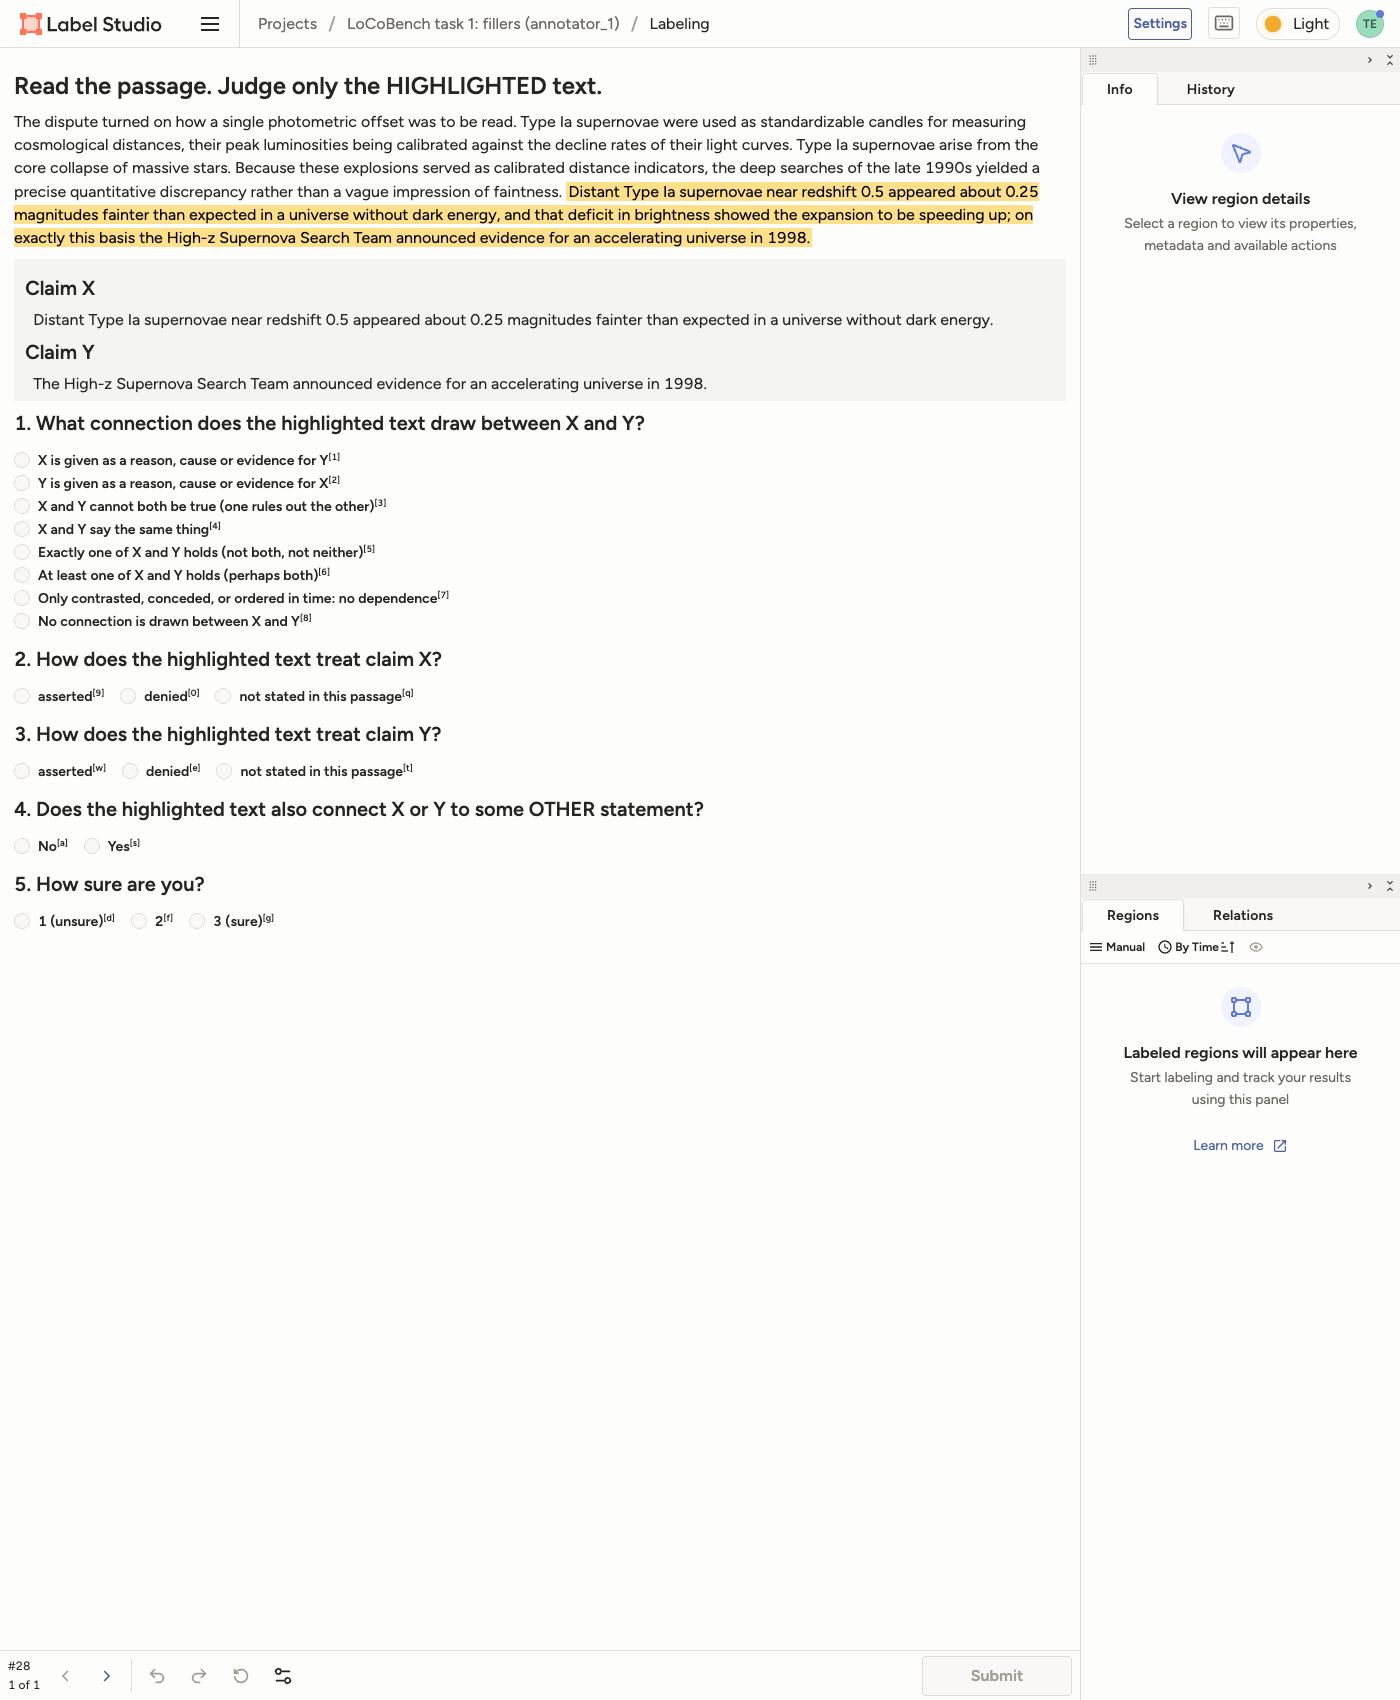
\includegraphics[width=0.9\textwidth,trim=0 755 325 45,clip]{figures/study_task1.png}}
\caption{\textbf{Task 1 in Label Studio}, as each annotator sees it locally: a filler
highlighted in its paragraph, the slot's two claims, and the five questions. Nothing on the screen
says which link was intended or whether the committee admitted the filler.}
\label{fig:study-ui}
\end{figure*}

\begin{figure*}[t]
\centering
\fbox{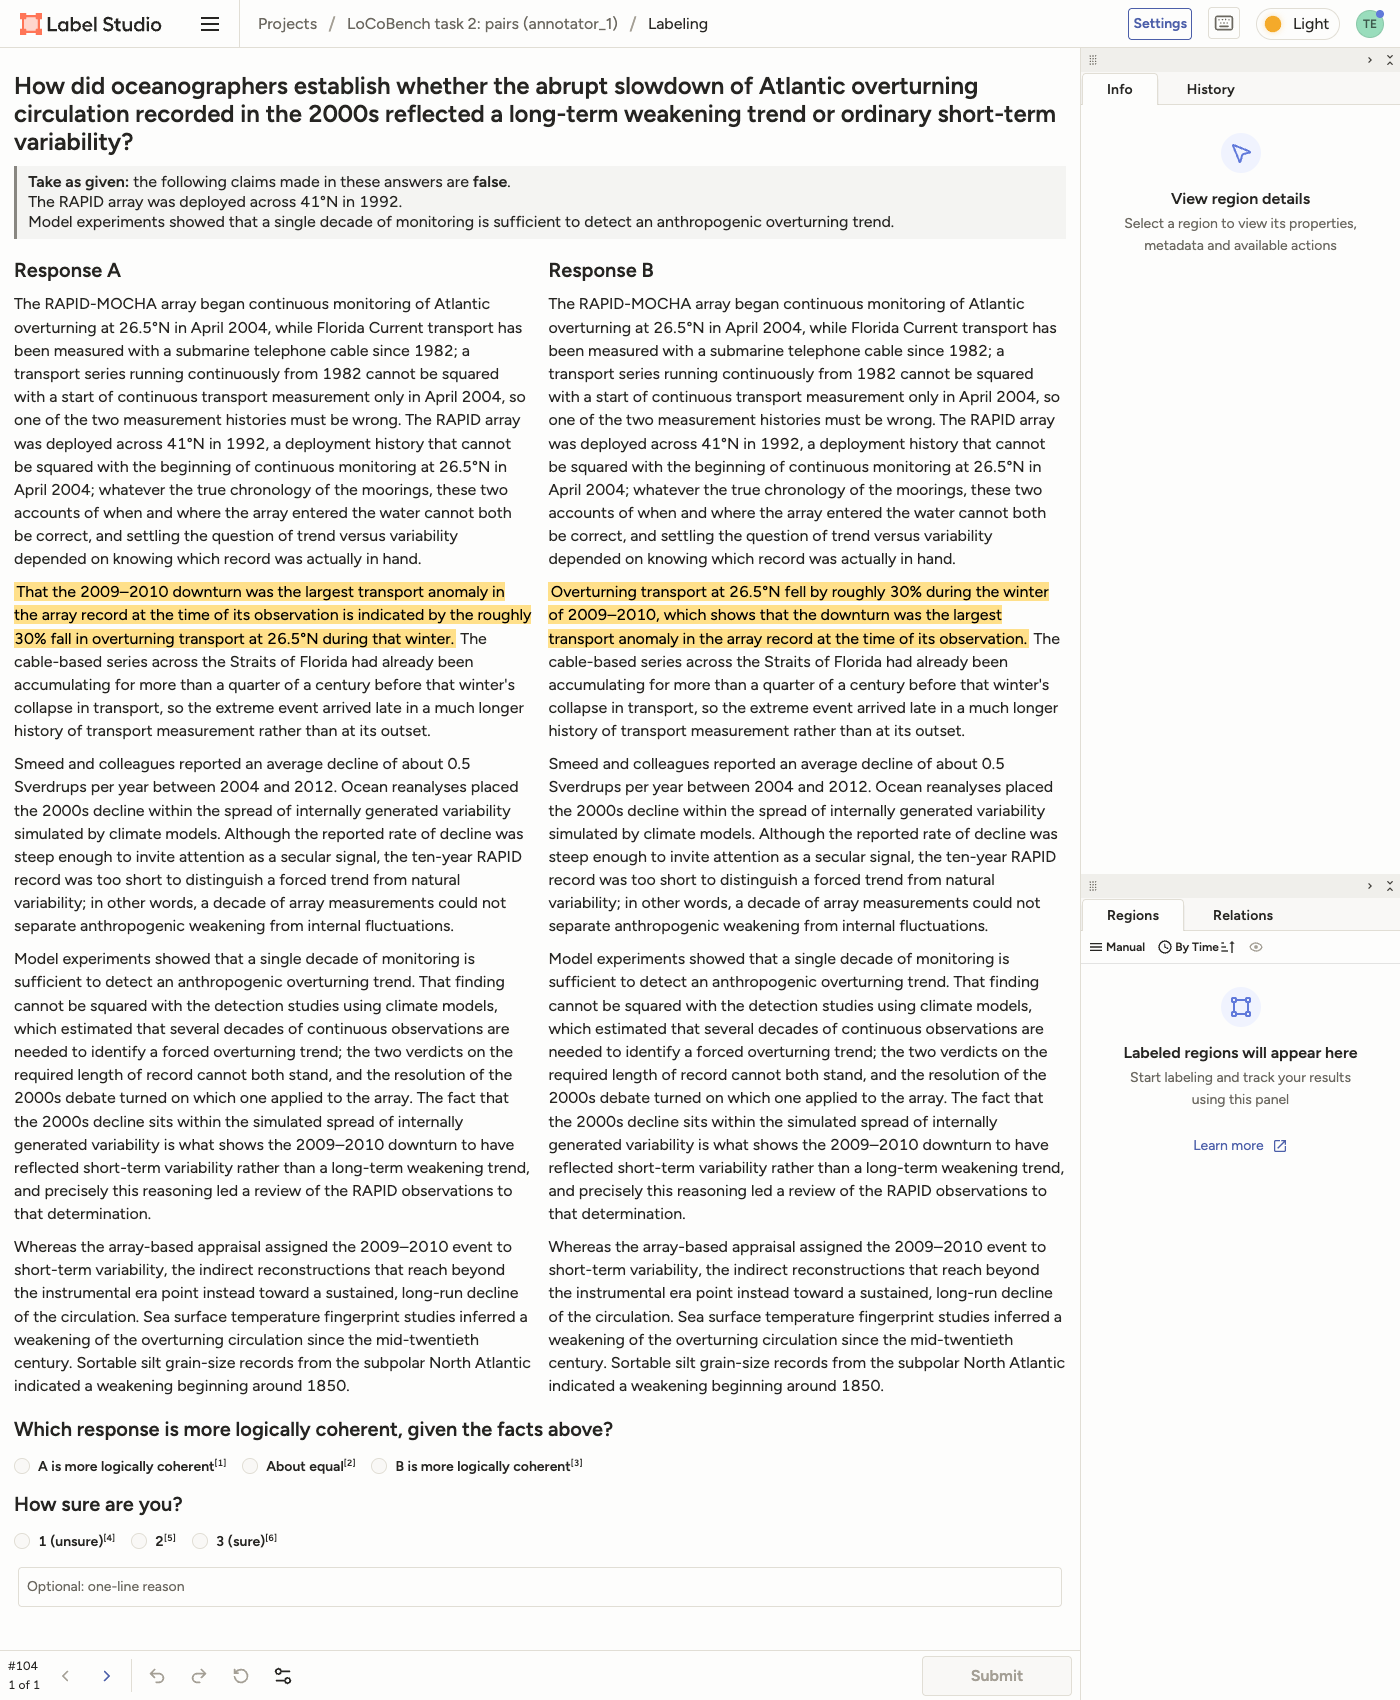
\includegraphics[width=0.9\textwidth,trim=0 520 325 45,clip]{figures/study_task2.png}}
\caption{\textbf{Task 2 in Label Studio} (top of the screen; the responses continue below, followed
by the preference, confidence and reason questions): the question, the family's false claims
given as facts, and two responses that differ only in the highlighted sentences.}
\label{fig:study-ui2}
\end{figure*}

Everything the study needs is generated by \texttt{scripts/locobench\_study\_build.py} from the
release and a fixed seed, and released with the paper:
\begin{itemize}[leftmargin=1.2em,itemsep=1pt,topsep=2pt]
\item one bundle per annotator, with its Task 1 and Task 2 files, the practice files, the two Label Studio labeling configurations, the annotator brief, setup
  instructions, the practice answers for the calibration discussion, and a script that creates
  the annotator's four projects in a local Label Studio;
\item the gold key, committed by hash in the pre-registration and never imported into Label
  Studio, which holds the sample, the intended answers, the committee's verdicts, the declared
  orders and the attention-check answers;
\item the pre-registration (hypotheses, sample, exclusions, scoring, power, consequences);
\item \texttt{scripts/locobench\_study\_analyze.py}, which checks the key against its hash,
  scores the Label Studio exports, and writes the report and the paper's macros. It was tested
  end to end on simulated exports, and on a real Label Studio instance (configuration validation,
  task import, annotation and JSON export), before annotation.
\end{itemize}

\paragraph{Task 1 options and their mapping.} The eight connection options map onto the
committee's SV5 labels: \emph{X is given as a reason, cause or evidence for Y} (and the reverse)
to the two directions of entailment; \emph{X and Y cannot both be true} to incompatibility;
\emph{say the same thing}, \emph{exactly one holds} and \emph{at least one holds} to equivalence,
exclusion and co-necessity; \emph{only contrasted, conceded, or ordered in time} and \emph{no
connection} to the no-factor readings, which score alike.

\paragraph{Budget.} Practice and calibration about 25 minutes, Task 1 about 75 minutes (72
fillers and 4 checks), Task 2 about two hours (18 families, 108 pairs and 2 checks), in sessions
of at most 90 minutes: 3.5--4 hours per annotator against a five-hour cap. \tbd{Measured times
and results.}
